% Options for packages loaded elsewhere
\PassOptionsToPackage{unicode}{hyperref}
\PassOptionsToPackage{hyphens}{url}
%
\documentclass[
]{article}
\usepackage{amsmath,amssymb}
\usepackage{lmodern}
\usepackage{ifxetex,ifluatex}
\ifnum 0\ifxetex 1\fi\ifluatex 1\fi=0 % if pdftex
  \usepackage[T1]{fontenc}
  \usepackage[utf8]{inputenc}
  \usepackage{textcomp} % provide euro and other symbols
\else % if luatex or xetex
  \usepackage{unicode-math}
  \defaultfontfeatures{Scale=MatchLowercase}
  \defaultfontfeatures[\rmfamily]{Ligatures=TeX,Scale=1}
\fi
% Use upquote if available, for straight quotes in verbatim environments
\IfFileExists{upquote.sty}{\usepackage{upquote}}{}
\IfFileExists{microtype.sty}{% use microtype if available
  \usepackage[]{microtype}
  \UseMicrotypeSet[protrusion]{basicmath} % disable protrusion for tt fonts
}{}
\makeatletter
\@ifundefined{KOMAClassName}{% if non-KOMA class
  \IfFileExists{parskip.sty}{%
    \usepackage{parskip}
  }{% else
    \setlength{\parindent}{0pt}
    \setlength{\parskip}{6pt plus 2pt minus 1pt}}
}{% if KOMA class
  \KOMAoptions{parskip=half}}
\makeatother
\usepackage{xcolor}
\IfFileExists{xurl.sty}{\usepackage{xurl}}{} % add URL line breaks if available
\IfFileExists{bookmark.sty}{\usepackage{bookmark}}{\usepackage{hyperref}}
\hypersetup{
  pdftitle={Crime and Topography in San Francisco},
  hidelinks,
  pdfcreator={LaTeX via pandoc}}
\urlstyle{same} % disable monospaced font for URLs
\usepackage[margin=1in]{geometry}
\usepackage{color}
\usepackage{fancyvrb}
\newcommand{\VerbBar}{|}
\newcommand{\VERB}{\Verb[commandchars=\\\{\}]}
\DefineVerbatimEnvironment{Highlighting}{Verbatim}{commandchars=\\\{\}}
% Add ',fontsize=\small' for more characters per line
\usepackage{framed}
\definecolor{shadecolor}{RGB}{248,248,248}
\newenvironment{Shaded}{\begin{snugshade}}{\end{snugshade}}
\newcommand{\AlertTok}[1]{\textcolor[rgb]{0.94,0.16,0.16}{#1}}
\newcommand{\AnnotationTok}[1]{\textcolor[rgb]{0.56,0.35,0.01}{\textbf{\textit{#1}}}}
\newcommand{\AttributeTok}[1]{\textcolor[rgb]{0.77,0.63,0.00}{#1}}
\newcommand{\BaseNTok}[1]{\textcolor[rgb]{0.00,0.00,0.81}{#1}}
\newcommand{\BuiltInTok}[1]{#1}
\newcommand{\CharTok}[1]{\textcolor[rgb]{0.31,0.60,0.02}{#1}}
\newcommand{\CommentTok}[1]{\textcolor[rgb]{0.56,0.35,0.01}{\textit{#1}}}
\newcommand{\CommentVarTok}[1]{\textcolor[rgb]{0.56,0.35,0.01}{\textbf{\textit{#1}}}}
\newcommand{\ConstantTok}[1]{\textcolor[rgb]{0.00,0.00,0.00}{#1}}
\newcommand{\ControlFlowTok}[1]{\textcolor[rgb]{0.13,0.29,0.53}{\textbf{#1}}}
\newcommand{\DataTypeTok}[1]{\textcolor[rgb]{0.13,0.29,0.53}{#1}}
\newcommand{\DecValTok}[1]{\textcolor[rgb]{0.00,0.00,0.81}{#1}}
\newcommand{\DocumentationTok}[1]{\textcolor[rgb]{0.56,0.35,0.01}{\textbf{\textit{#1}}}}
\newcommand{\ErrorTok}[1]{\textcolor[rgb]{0.64,0.00,0.00}{\textbf{#1}}}
\newcommand{\ExtensionTok}[1]{#1}
\newcommand{\FloatTok}[1]{\textcolor[rgb]{0.00,0.00,0.81}{#1}}
\newcommand{\FunctionTok}[1]{\textcolor[rgb]{0.00,0.00,0.00}{#1}}
\newcommand{\ImportTok}[1]{#1}
\newcommand{\InformationTok}[1]{\textcolor[rgb]{0.56,0.35,0.01}{\textbf{\textit{#1}}}}
\newcommand{\KeywordTok}[1]{\textcolor[rgb]{0.13,0.29,0.53}{\textbf{#1}}}
\newcommand{\NormalTok}[1]{#1}
\newcommand{\OperatorTok}[1]{\textcolor[rgb]{0.81,0.36,0.00}{\textbf{#1}}}
\newcommand{\OtherTok}[1]{\textcolor[rgb]{0.56,0.35,0.01}{#1}}
\newcommand{\PreprocessorTok}[1]{\textcolor[rgb]{0.56,0.35,0.01}{\textit{#1}}}
\newcommand{\RegionMarkerTok}[1]{#1}
\newcommand{\SpecialCharTok}[1]{\textcolor[rgb]{0.00,0.00,0.00}{#1}}
\newcommand{\SpecialStringTok}[1]{\textcolor[rgb]{0.31,0.60,0.02}{#1}}
\newcommand{\StringTok}[1]{\textcolor[rgb]{0.31,0.60,0.02}{#1}}
\newcommand{\VariableTok}[1]{\textcolor[rgb]{0.00,0.00,0.00}{#1}}
\newcommand{\VerbatimStringTok}[1]{\textcolor[rgb]{0.31,0.60,0.02}{#1}}
\newcommand{\WarningTok}[1]{\textcolor[rgb]{0.56,0.35,0.01}{\textbf{\textit{#1}}}}
\usepackage{graphicx}
\makeatletter
\def\maxwidth{\ifdim\Gin@nat@width>\linewidth\linewidth\else\Gin@nat@width\fi}
\def\maxheight{\ifdim\Gin@nat@height>\textheight\textheight\else\Gin@nat@height\fi}
\makeatother
% Scale images if necessary, so that they will not overflow the page
% margins by default, and it is still possible to overwrite the defaults
% using explicit options in \includegraphics[width, height, ...]{}
\setkeys{Gin}{width=\maxwidth,height=\maxheight,keepaspectratio}
% Set default figure placement to htbp
\makeatletter
\def\fps@figure{htbp}
\makeatother
\setlength{\emergencystretch}{3em} % prevent overfull lines
\providecommand{\tightlist}{%
  \setlength{\itemsep}{0pt}\setlength{\parskip}{0pt}}
\setcounter{secnumdepth}{-\maxdimen} % remove section numbering
\usepackage{booktabs}
\usepackage{longtable}
\usepackage{array}
\usepackage{multirow}
\usepackage{wrapfig}
\usepackage{float}
\usepackage{colortbl}
\usepackage{pdflscape}
\usepackage{tabu}
\usepackage{threeparttable}
\usepackage{threeparttablex}
\usepackage[normalem]{ulem}
\usepackage{makecell}
\usepackage{xcolor}
\ifluatex
  \usepackage{selnolig}  % disable illegal ligatures
\fi
\newlength{\cslhangindent}
\setlength{\cslhangindent}{1.5em}
\newlength{\csllabelwidth}
\setlength{\csllabelwidth}{3em}
\newenvironment{CSLReferences}[2] % #1 hanging-ident, #2 entry spacing
 {% don't indent paragraphs
  \setlength{\parindent}{0pt}
  % turn on hanging indent if param 1 is 1
  \ifodd #1 \everypar{\setlength{\hangindent}{\cslhangindent}}\ignorespaces\fi
  % set entry spacing
  \ifnum #2 > 0
  \setlength{\parskip}{#2\baselineskip}
  \fi
 }%
 {}
\usepackage{calc}
\newcommand{\CSLBlock}[1]{#1\hfill\break}
\newcommand{\CSLLeftMargin}[1]{\parbox[t]{\csllabelwidth}{#1}}
\newcommand{\CSLRightInline}[1]{\parbox[t]{\linewidth - \csllabelwidth}{#1}\break}
\newcommand{\CSLIndent}[1]{\hspace{\cslhangindent}#1}

\title{Crime and Topography in San Francisco}
\author{true}
\date{2021-11-02}

\begin{document}
\maketitle

That is one steep street!

\hypertarget{analysis-plan}{%
\subsection{Analysis Plan}\label{analysis-plan}}

This analysis will follow the specific steps outlined in Table 1 below:

\begin{Shaded}
\begin{Highlighting}[]
\FunctionTok{data.frame}\NormalTok{(}\StringTok{"Step"} \OtherTok{=} \FunctionTok{c}\NormalTok{(}\DecValTok{1}\SpecialCharTok{:}\DecValTok{8}\NormalTok{),}
           \StringTok{"Description"} \OtherTok{=} \FunctionTok{c}\NormalTok{(}\StringTok{"Identify research question"}\NormalTok{, }
                             \StringTok{"Select key variables"}\NormalTok{,}
                             \StringTok{"Collect data"}\NormalTok{,}
                             \StringTok{"Describe data"}\NormalTok{,}
                             \StringTok{"Visualize relationships"}\NormalTok{,}
                             \StringTok{"Test OLS assumptions"}\NormalTok{,}
                             \StringTok{"Conduct regression analysis"}\NormalTok{,}
                             \StringTok{"Interpret results"}\NormalTok{)) }\SpecialCharTok{\%\textgreater{}\%} 
  \FunctionTok{kable}\NormalTok{(}\AttributeTok{caption =} \StringTok{"Analysis Plan"}\NormalTok{) }\SpecialCharTok{\%\textgreater{}\%}
  \FunctionTok{kable\_paper}\NormalTok{(}\AttributeTok{full\_width =} \ConstantTok{FALSE}\NormalTok{) }\SpecialCharTok{\%\textgreater{}\%}
  \FunctionTok{kable\_styling}\NormalTok{(}\AttributeTok{latex\_options =} \StringTok{"striped"}\NormalTok{,}
                \AttributeTok{font\_size =} \DecValTok{15}\NormalTok{) }\SpecialCharTok{\%\textgreater{}\%} 
  \FunctionTok{column\_spec}\NormalTok{(}\DecValTok{1}\NormalTok{, }\AttributeTok{bold =}\NormalTok{ T) }\SpecialCharTok{\%\textgreater{}\%}
  \FunctionTok{row\_spec}\NormalTok{(}\DecValTok{0}\NormalTok{, }\AttributeTok{bold =}\NormalTok{ T, }\AttributeTok{color =} \StringTok{"black"}\NormalTok{)}
\end{Highlighting}
\end{Shaded}

\begin{table}

\caption{\label{tab:unnamed-chunk-1}Analysis Plan}
\centering
\fontsize{15}{17}\selectfont
\begin{tabular}[t]{>{}r|l}
\hline
\textcolor{black}{\textbf{Step}} & \textcolor{black}{\textbf{Description}}\\
\hline
\textbf{\cellcolor{gray!6}{1}} & \cellcolor{gray!6}{Identify research question}\\
\hline
\textbf{2} & Select key variables\\
\hline
\textbf{\cellcolor{gray!6}{3}} & \cellcolor{gray!6}{Collect data}\\
\hline
\textbf{4} & Describe data\\
\hline
\textbf{\cellcolor{gray!6}{5}} & \cellcolor{gray!6}{Visualize relationships}\\
\hline
\textbf{6} & Test OLS assumptions\\
\hline
\textbf{\cellcolor{gray!6}{7}} & \cellcolor{gray!6}{Conduct regression analysis}\\
\hline
\textbf{8} & Interpret results\\
\hline
\end{tabular}
\end{table}

\hypertarget{research-question}{%
\subsection{1. Research Question}\label{research-question}}

My research question is: \textbf{What is the relationship between
topography and car break-ins in San Francisco?}

\hypertarget{background}{%
\subsubsection{Background}\label{background}}

Both terrain and motor vehicle crimes are ubiquitous when discussing
living or visiting San Francisco. In April 2021, Young-An Kim \& James
C. Wo published
\href{https://www.tandfonline.com/doi/full/10.1080/07352166.2021.1901591}{Topography
and crime in place: The effects of elevation, slope, and betweenness in
San Francisco street segments}. This study supports the idea that
``hilliness'' has an effect on crime, taking into consideration
socio-economic characteristics Kim and Wo (2021). However, their
analysis did not separate by specific crime categories and instead
included all types of crime, including violent, nonviolent, property,
etc.

\textbf{My analysis will focus only on car break-ins rather than all
crime reports}, as I believe that these crimes will have a more
significant relationship with topography. In addition, my analysis will
use more recent crime report and socio-economic data sets. Understanding
the relationship between topography and car break-ins can influence
local-level policy decisions and direct limited resources dedicated to
crime prevention. For example, the city could focus enforcement and
policy on areas within certain elevation and slope ranges that are
identified in this analysis as being particularly susceptible to car
break-ins.

\hypertarget{select-key-variables}{%
\subsection{2. Select key variables}\label{select-key-variables}}

Table 2 below contains the key measures of interest in our analysis:

\begin{Shaded}
\begin{Highlighting}[]
\FunctionTok{data.frame}\NormalTok{(}\StringTok{"Dependent Variable"} \OtherTok{=} \FunctionTok{c}\NormalTok{(}\StringTok{"Number of Car Break{-}Ins"}\NormalTok{, }\StringTok{""}\NormalTok{),}
           \StringTok{"Independent Variables"} \OtherTok{=} \FunctionTok{c}\NormalTok{(}\StringTok{"Elevation"}\NormalTok{, }\StringTok{"Slope"}\NormalTok{), }
           \StringTok{"Control Variable"} \OtherTok{=} \FunctionTok{c}\NormalTok{(}\StringTok{"Median Income"}\NormalTok{,}\StringTok{""}\NormalTok{)) }\SpecialCharTok{\%\textgreater{}\%} 
  \FunctionTok{kable}\NormalTok{(}\AttributeTok{col.names =} \FunctionTok{c}\NormalTok{(}\StringTok{"Dependent Variable"}\NormalTok{, }\StringTok{"Independent Variables"}\NormalTok{, }\StringTok{"Control Variable"}\NormalTok{), }\AttributeTok{caption =} \StringTok{"Key variables for regression analysis"}\NormalTok{) }\SpecialCharTok{\%\textgreater{}\%}
  \FunctionTok{kable\_paper}\NormalTok{(}\AttributeTok{full\_width =} \ConstantTok{FALSE}\NormalTok{) }\SpecialCharTok{\%\textgreater{}\%}
  \FunctionTok{kable\_styling}\NormalTok{(}\AttributeTok{latex\_options =} \StringTok{"striped"}\NormalTok{,}
                \AttributeTok{font\_size =} \DecValTok{15}\NormalTok{) }\SpecialCharTok{\%\textgreater{}\%} 
  \FunctionTok{column\_spec}\NormalTok{(}\DecValTok{1}\NormalTok{, }\AttributeTok{bold =}\NormalTok{ T) }\SpecialCharTok{\%\textgreater{}\%}
  \FunctionTok{row\_spec}\NormalTok{(}\DecValTok{0}\NormalTok{, }\AttributeTok{bold =}\NormalTok{ T, }\AttributeTok{color =} \StringTok{"black"}\NormalTok{)}
\end{Highlighting}
\end{Shaded}

\begin{table}

\caption{\label{tab:unnamed-chunk-2}Key variables for regression analysis}
\centering
\fontsize{15}{17}\selectfont
\begin{tabular}[t]{>{}l|l|l}
\hline
\textcolor{black}{\textbf{Dependent Variable}} & \textcolor{black}{\textbf{Independent Variables}} & \textcolor{black}{\textbf{Control Variable}}\\
\hline
\textbf{\cellcolor{gray!6}{Number of Car Break-Ins}} & \cellcolor{gray!6}{Elevation} & \cellcolor{gray!6}{Median Income}\\
\hline
\textbf{} & Slope & \\
\hline
\end{tabular}
\end{table}

When discussing topography, both elevation and slope are necessary for
inclusion because these two capture the effect of local level
topography. In any econometric analysis, it is vital to control for
socio-economic variables. Thus, median income is included as a control
variable.

Here is the regression equation:

\[NumBreakIns_i = \beta_0 + \beta_1Elevation_i + \beta_2Slope_i + \beta_3MedianIncome_i + u_i\]

Based on the existing literature by Kim \& Wo, \textbf{it is expected
that there is a negative correlation between number of car break-ins and
all three independent variables}.

\hypertarget{collect-data}{%
\subsection{3. Collect data}\label{collect-data}}

\begin{itemize}
\tightlist
\item
  \textbf{Crime} (City and San Francisco (2021))

  \begin{itemize}
  \tightlist
  \item
    Retrieved from the
    \href{https://data.sfgov.org/Public-Safety/Police-Department-Incident-Reports-2018-to-Present/wg3w-h783}{San
    Francisco Open Data Portal}
  \item
    All crime reports from 2018-01-01 to 2021-11-04.

    \begin{itemize}
    \tightlist
    \item
      Queried to only include ``Motor Vehicle Theft''
    \end{itemize}
  \item
    Locations are aggregated to closest street intersections.
  \end{itemize}
\item
  \textbf{Elevation contours} (City and San Francisco (2021))

  \begin{itemize}
  \tightlist
  \item
    Retrieved from the
    \href{https://data.sfgov.org/Energy-and-Environment/Elevation-Contours/rnbg-2qxw}{San
    Francisco Open Data Portal}
  \item
    5 ft. elevation contours
  \item
    Used directly for \textbf{elevation} and also to derive
    \textbf{slope} through a geo-processing workflow in QGIS with GRASS
    (see \href{https://www.youtube.com/watch?v=MvnW6w1_yJg}{this video}
    for details on this process).
  \end{itemize}
\item
  \textbf{Median income} (Walker (2021))

  \begin{itemize}
  \tightlist
  \item
    Retrieved through the \texttt{tidycensus} package via the
    \href{https://www.census.gov/data/developers/data-sets.html}{US
    Census Bureau}.
  \item
    census Tract detail level from the 5-year 2015-2019 ACS data.
  \end{itemize}
\end{itemize}

Since our variables interact over space, we merge the crimes,
topography, and median income data sets by spatially joining them
together. All data sets are loaded into \texttt{R} as
\textbf{shapefiles} in the Coordinate Reference System (CRS) EPSG:7132
(NAD83(2011) / San Francisco CS13 (ftUS)), which is a projected CRS for
the city and county of San Francisco adequate for high-precision (0.03
ft) analysis.

\begin{Shaded}
\begin{Highlighting}[]
\CommentTok{\# Find index of nearest contour to each crime}
\NormalTok{elev }\OtherTok{\textless{}{-}} \FunctionTok{st\_nearest\_feature}\NormalTok{(}\AttributeTok{x =}\NormalTok{ crimes, }\AttributeTok{y =}\NormalTok{ contours)}

\CommentTok{\# Add elevation and binary slope columns}
\NormalTok{crimes }\OtherTok{\textless{}{-}}\NormalTok{ crimes }\SpecialCharTok{\%\textgreater{}\%} 
  \FunctionTok{st\_join}\NormalTok{(}\AttributeTok{y =}\NormalTok{ census\_geom, }\AttributeTok{join =}\NormalTok{ st\_within, }\AttributeTok{left =} \ConstantTok{TRUE}\NormalTok{) }\SpecialCharTok{\%\textgreater{}\%} 
  \FunctionTok{mutate}\NormalTok{(}\AttributeTok{elev =}\NormalTok{ contours[elev,]}\SpecialCharTok{$}\NormalTok{elevation) }\SpecialCharTok{\%\textgreater{}\%} 
  \FunctionTok{rename}\NormalTok{(}\AttributeTok{median\_income =}\NormalTok{ estimate) }\SpecialCharTok{\%\textgreater{}\%} 
  \FunctionTok{select}\NormalTok{(date\_incid, slope, median\_income, elev, geometry)}

\CommentTok{\# Group by all three variables}
\NormalTok{crimes\_summary }\OtherTok{\textless{}{-}}\NormalTok{ crimes }\SpecialCharTok{\%\textgreater{}\%} 
  \FunctionTok{st\_drop\_geometry}\NormalTok{() }\SpecialCharTok{\%\textgreater{}\%} 
  \FunctionTok{group\_by}\NormalTok{(slope, median\_income, elev) }\SpecialCharTok{\%\textgreater{}\%} 
  \FunctionTok{summarize}\NormalTok{(}\AttributeTok{count =} \FunctionTok{n}\NormalTok{())}
\end{Highlighting}
\end{Shaded}

\hypertarget{describe-data}{%
\subsection{4. Describe data}\label{describe-data}}

The summary statistics for the data are provided in Table 3 below.

\begin{Shaded}
\begin{Highlighting}[]
\NormalTok{crimes }\SpecialCharTok{\%\textgreater{}\%} 
  \FunctionTok{st\_drop\_geometry}\NormalTok{() }\SpecialCharTok{\%\textgreater{}\%} 
  \FunctionTok{select}\NormalTok{(slope, elev, median\_income) }\SpecialCharTok{\%\textgreater{}\%} 
\NormalTok{  psych}\SpecialCharTok{::}\FunctionTok{describe}\NormalTok{(}\AttributeTok{fast=}\ConstantTok{TRUE}\NormalTok{) }\SpecialCharTok{\%\textgreater{}\%} 
  \FunctionTok{kable}\NormalTok{(}\AttributeTok{col.names =} \FunctionTok{c}\NormalTok{(}\StringTok{""}\NormalTok{, }\StringTok{"Count"}\NormalTok{, }\StringTok{"Mean"}\NormalTok{, }\StringTok{"SD"}\NormalTok{, }\StringTok{"Min"}\NormalTok{, }\StringTok{"Max"}\NormalTok{, }\StringTok{"Range"}\NormalTok{, }\StringTok{"SE"}\NormalTok{), }\AttributeTok{caption =} \StringTok{"Summary statistics for Slope, Elevation, and Median Income variables"}\NormalTok{) }\SpecialCharTok{\%\textgreater{}\%}
  \FunctionTok{kable\_paper}\NormalTok{(}\AttributeTok{full\_width =} \ConstantTok{FALSE}\NormalTok{) }\SpecialCharTok{\%\textgreater{}\%}
  \FunctionTok{kable\_styling}\NormalTok{(}\AttributeTok{latex\_options =} \StringTok{"striped"}\NormalTok{,}
                \AttributeTok{font\_size =} \DecValTok{15}\NormalTok{) }\SpecialCharTok{\%\textgreater{}\%} 
  \FunctionTok{column\_spec}\NormalTok{(}\DecValTok{1}\NormalTok{, }\AttributeTok{bold =}\NormalTok{ T) }\SpecialCharTok{\%\textgreater{}\%}
  \FunctionTok{row\_spec}\NormalTok{(}\DecValTok{0}\NormalTok{, }\AttributeTok{bold =}\NormalTok{ T, }\AttributeTok{color =} \StringTok{"black"}\NormalTok{)}
\end{Highlighting}
\end{Shaded}

\begin{table}

\caption{\label{tab:unnamed-chunk-3}Summary statistics for Slope, Elevation, and Median Income variables}
\centering
\fontsize{15}{17}\selectfont
\begin{tabular}[t]{>{}l|r|r|r|r|r|r|r|r}
\hline
\textcolor{black}{\textbf{ }} & \textcolor{black}{\textbf{}} & \textcolor{black}{\textbf{Count}} & \textcolor{black}{\textbf{Mean}} & \textcolor{black}{\textbf{SD}} & \textcolor{black}{\textbf{Min}} & \textcolor{black}{\textbf{Max}} & \textcolor{black}{\textbf{Range}} & \textcolor{black}{\textbf{SE}}\\
\hline
\textbf{\cellcolor{gray!6}{slope}} & \cellcolor{gray!6}{1} & \cellcolor{gray!6}{24454} & \cellcolor{gray!6}{4.492966} & \cellcolor{gray!6}{4.793824} & \cellcolor{gray!6}{0} & \cellcolor{gray!6}{68} & \cellcolor{gray!6}{68} & \cellcolor{gray!6}{0.0306554}\\
\hline
\textbf{elev} & 2 & 24454 & 129.321379 & 120.439659 & -5 & 780 & 785 & 0.7701841\\
\hline
\textbf{\cellcolor{gray!6}{median\_income}} & \cellcolor{gray!6}{3} & \cellcolor{gray!6}{23764} & \cellcolor{gray!6}{114039.269567} & \cellcolor{gray!6}{47501.416992} & \cellcolor{gray!6}{12340} & \cellcolor{gray!6}{208425} & \cellcolor{gray!6}{196085} & \cellcolor{gray!6}{308.1390882}\\
\hline
\end{tabular}
\end{table}

We can see in the \textbf{count} column that there are 24,454 total
break-ins in our data, with some missing values for median income. The
\textbf{slope} ranges from 0 to 68 percent (\textasciitilde34 degrees)
with a mean value of approximately 4.5 percent. This indicates that
there are vastly more break-ins on flatter streets as expected. The
\textbf{elevation} ranges from -5 to 780 feet with a mean value of
approximately 130 (note: negative values are a result of attaching the
nearest contour level to crimes very close to the coastline). Again,
there are more break-ins at lower elevations than higher. The
\textbf{median income} ranges from \textasciitilde\$12,000 to
\textasciitilde\$208,000 with a mean value of approximately \$114,000.
This indicates that our median income data appears to be somewhat evenly
distributed.

The box plots below visualize these observations:

\begin{Shaded}
\begin{Highlighting}[]
\NormalTok{slope\_box }\OtherTok{\textless{}{-}} \FunctionTok{ggplot}\NormalTok{(}\AttributeTok{data =}\NormalTok{ crimes, }\FunctionTok{aes}\NormalTok{(}\AttributeTok{x =} \StringTok{""}\NormalTok{, }\AttributeTok{y =}\NormalTok{ slope)) }\SpecialCharTok{+}
  \FunctionTok{geom\_boxplot}\NormalTok{(}\AttributeTok{color =} \StringTok{"orange"}\NormalTok{) }\SpecialCharTok{+}
  \FunctionTok{geom\_jitter}\NormalTok{(}\FunctionTok{aes}\NormalTok{(}\AttributeTok{color =}\NormalTok{ slope), }
              \AttributeTok{width =} \FloatTok{0.2}\NormalTok{,}
              \AttributeTok{size=}\FloatTok{0.4}\NormalTok{, }
              \AttributeTok{alpha=}\FloatTok{0.025}\NormalTok{, }
              \AttributeTok{show.legend =} \ConstantTok{FALSE}\NormalTok{) }\SpecialCharTok{+}
  \FunctionTok{theme\_classic}\NormalTok{() }\SpecialCharTok{+}
  \FunctionTok{theme}\NormalTok{(}\AttributeTok{axis.text.x =} \FunctionTok{element\_blank}\NormalTok{(),}
        \AttributeTok{axis.ticks.x =} \FunctionTok{element\_blank}\NormalTok{(),}
        \AttributeTok{axis.title.y =} \FunctionTok{element\_blank}\NormalTok{()) }\SpecialCharTok{+}
  \FunctionTok{labs}\NormalTok{(}\AttributeTok{x =} \StringTok{"Slope (percent)"}\NormalTok{)}

\NormalTok{elev\_box }\OtherTok{\textless{}{-}} \FunctionTok{ggplot}\NormalTok{(}\AttributeTok{data =}\NormalTok{ crimes, }\FunctionTok{aes}\NormalTok{(}\AttributeTok{x =} \StringTok{""}\NormalTok{, }\AttributeTok{y =}\NormalTok{ elev)) }\SpecialCharTok{+}
  \FunctionTok{geom\_boxplot}\NormalTok{(}\AttributeTok{color =} \StringTok{"darkgreen"}\NormalTok{) }\SpecialCharTok{+}
  \FunctionTok{geom\_jitter}\NormalTok{(}\FunctionTok{aes}\NormalTok{(}\AttributeTok{color =}\NormalTok{ elev), }
              \AttributeTok{width =} \FloatTok{0.2}\NormalTok{,}
              \AttributeTok{size=}\FloatTok{0.4}\NormalTok{, }
              \AttributeTok{alpha=}\FloatTok{0.025}\NormalTok{, }
              \AttributeTok{show.legend =} \ConstantTok{FALSE}\NormalTok{) }\SpecialCharTok{+}
  \FunctionTok{theme\_classic}\NormalTok{() }\SpecialCharTok{+}
  \FunctionTok{theme}\NormalTok{(}\AttributeTok{axis.text.x =} \FunctionTok{element\_blank}\NormalTok{(),}
        \AttributeTok{axis.ticks.x =} \FunctionTok{element\_blank}\NormalTok{(),}
        \AttributeTok{axis.title.y =} \FunctionTok{element\_blank}\NormalTok{()) }\SpecialCharTok{+}
  \FunctionTok{labs}\NormalTok{(}\AttributeTok{x =} \StringTok{"Elevation (feet)"}\NormalTok{)}

\NormalTok{income\_box }\OtherTok{\textless{}{-}} \FunctionTok{ggplot}\NormalTok{(}\AttributeTok{data =}\NormalTok{ crimes, }\FunctionTok{aes}\NormalTok{(}\AttributeTok{x =} \StringTok{""}\NormalTok{, }\AttributeTok{y =}\NormalTok{ median\_income)) }\SpecialCharTok{+}
  \FunctionTok{geom\_boxplot}\NormalTok{(}\AttributeTok{color =} \StringTok{"blue"}\NormalTok{) }\SpecialCharTok{+}
  \FunctionTok{geom\_jitter}\NormalTok{(}\FunctionTok{aes}\NormalTok{(}\AttributeTok{color =}\NormalTok{ median\_income), }
              \AttributeTok{width =} \FloatTok{0.2}\NormalTok{,}
              \AttributeTok{size=}\FloatTok{0.4}\NormalTok{, }
              \AttributeTok{alpha=}\FloatTok{0.025}\NormalTok{, }
              \AttributeTok{show.legend =} \ConstantTok{FALSE}\NormalTok{) }\SpecialCharTok{+}
  \FunctionTok{theme\_classic}\NormalTok{() }\SpecialCharTok{+}
  \FunctionTok{theme}\NormalTok{(}\AttributeTok{axis.text.x =} \FunctionTok{element\_blank}\NormalTok{(),}
        \AttributeTok{axis.ticks.x =} \FunctionTok{element\_blank}\NormalTok{(),}
        \AttributeTok{axis.title.y =} \FunctionTok{element\_blank}\NormalTok{()) }\SpecialCharTok{+}
  \FunctionTok{labs}\NormalTok{(}\AttributeTok{x =} \StringTok{"Median Income (USD)"}\NormalTok{)}

\NormalTok{elev\_box }\SpecialCharTok{+}\NormalTok{ slope\_box }\SpecialCharTok{+}\NormalTok{ income\_box }\SpecialCharTok{+} \FunctionTok{plot\_annotation}\NormalTok{(}\AttributeTok{title =} \StringTok{\textquotesingle{}Figure 1. Boxplots of Independent Variables\textquotesingle{}}\NormalTok{,}
                                                    \AttributeTok{theme =} \FunctionTok{theme}\NormalTok{(}\AttributeTok{plot.title =} \FunctionTok{element\_text}\NormalTok{(}\AttributeTok{hjust =} \FloatTok{0.5}\NormalTok{)))}
\end{Highlighting}
\end{Shaded}

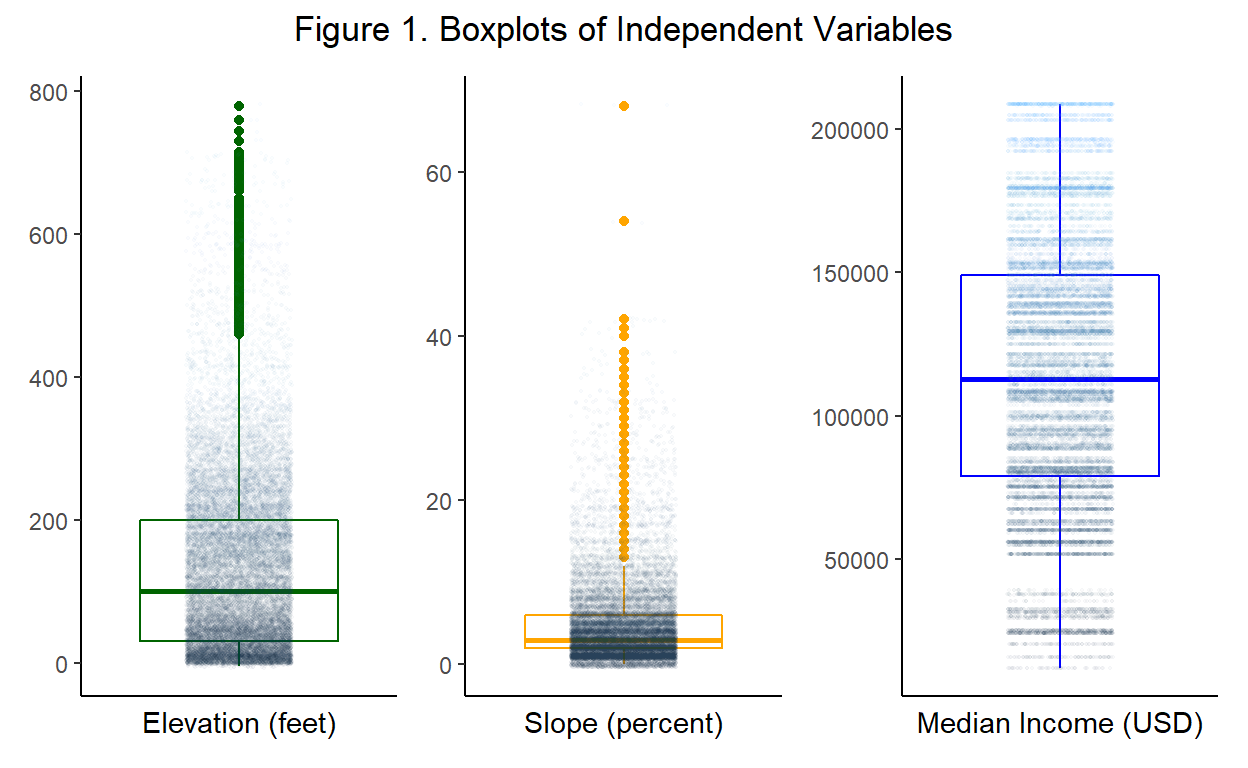
\includegraphics{sf-crime-and-hilliness_files/figure-latex/unnamed-chunk-4-1.pdf}

The box plots more clearly demonstrate that both elevation and slope
have more occurrences at low values than high values, with high
outliers. These extreme values appear to be accurate - the highest peak
in San Francisco is Mount Davidson at 938 feet and the steepest surveyed
road is Bradford Street at 41\% grade. This indicates that two of the
slope outliers are likely due to data artifacts.

\hypertarget{visualize-relationships}{%
\subsection{5. Visualize relationships}\label{visualize-relationships}}

The following plots in Figure 2 show the simple relationships between
count of car break ins and the three independent variables (elevation,
slope, and median income).

\begin{Shaded}
\begin{Highlighting}[]
\CommentTok{\# Group by income}
\NormalTok{income\_summary }\OtherTok{\textless{}{-}}\NormalTok{ crimes }\SpecialCharTok{\%\textgreater{}\%} 
  \FunctionTok{st\_drop\_geometry}\NormalTok{() }\SpecialCharTok{\%\textgreater{}\%} 
  \FunctionTok{group\_by}\NormalTok{(median\_income) }\SpecialCharTok{\%\textgreater{}\%} 
  \FunctionTok{summarize}\NormalTok{(}\AttributeTok{count =} \FunctionTok{n}\NormalTok{())}

\NormalTok{income\_plot }\OtherTok{=} \FunctionTok{ggplot}\NormalTok{(}\AttributeTok{data =}\NormalTok{ income\_summary, }\FunctionTok{aes}\NormalTok{(}\AttributeTok{x =}\NormalTok{ median\_income, }\AttributeTok{y =}\NormalTok{ count)) }\SpecialCharTok{+}
  \FunctionTok{geom\_point}\NormalTok{(}\AttributeTok{alpha =} \FloatTok{0.5}\NormalTok{, }\AttributeTok{color =} \StringTok{"darkgreen"}\NormalTok{) }\SpecialCharTok{+}
  \FunctionTok{geom\_smooth}\NormalTok{(}\AttributeTok{method =} \StringTok{"lm"}\NormalTok{, }\AttributeTok{se =} \ConstantTok{FALSE}\NormalTok{) }\SpecialCharTok{+}
  \FunctionTok{theme\_classic}\NormalTok{() }\SpecialCharTok{+}
  \FunctionTok{labs}\NormalTok{(}\AttributeTok{title =} \StringTok{"Crime and Median Income"}\NormalTok{,}
       \AttributeTok{x =} \StringTok{"Median Income (USD)"}\NormalTok{,}
       \AttributeTok{y =} \StringTok{"Number of Break{-}Ins"}\NormalTok{) }\SpecialCharTok{+}
  \FunctionTok{theme}\NormalTok{(}\AttributeTok{title =} \FunctionTok{element\_text}\NormalTok{(}\AttributeTok{size =} \DecValTok{10}\NormalTok{))}

\CommentTok{\# Group by elevation}
\NormalTok{elev\_summary }\OtherTok{\textless{}{-}}\NormalTok{ crimes }\SpecialCharTok{\%\textgreater{}\%} 
  \FunctionTok{st\_drop\_geometry}\NormalTok{() }\SpecialCharTok{\%\textgreater{}\%} 
  \FunctionTok{group\_by}\NormalTok{(elev) }\SpecialCharTok{\%\textgreater{}\%} 
  \FunctionTok{summarize}\NormalTok{(}\AttributeTok{count =} \FunctionTok{n}\NormalTok{())}

\NormalTok{elev\_plot }\OtherTok{\textless{}{-}} \FunctionTok{ggplot}\NormalTok{(}\AttributeTok{data =}\NormalTok{ elev\_summary, }\FunctionTok{aes}\NormalTok{(}\AttributeTok{x =}\NormalTok{ elev, }\AttributeTok{y =}\NormalTok{ count)) }\SpecialCharTok{+}
  \FunctionTok{geom\_point}\NormalTok{(}\AttributeTok{alpha =} \FloatTok{0.5}\NormalTok{, }\AttributeTok{color =} \StringTok{"orange"}\NormalTok{) }\SpecialCharTok{+}
  \FunctionTok{geom\_smooth}\NormalTok{(}\AttributeTok{method =} \StringTok{"lm"}\NormalTok{, }\AttributeTok{se =} \ConstantTok{FALSE}\NormalTok{) }\SpecialCharTok{+}
  \FunctionTok{theme\_classic}\NormalTok{() }\SpecialCharTok{+}
  \FunctionTok{labs}\NormalTok{(}\AttributeTok{title =} \StringTok{"Crime and Elevation"}\NormalTok{,}
       \AttributeTok{x =} \StringTok{"Elevation (feet)"}\NormalTok{,}
       \AttributeTok{y =} \StringTok{"Number of Break{-}Ins"}\NormalTok{) }\SpecialCharTok{+}
  \FunctionTok{theme}\NormalTok{(}\AttributeTok{title =} \FunctionTok{element\_text}\NormalTok{(}\AttributeTok{size =} \DecValTok{10}\NormalTok{))}

\CommentTok{\# Group by slope}
\NormalTok{slope\_summary }\OtherTok{\textless{}{-}}\NormalTok{ crimes }\SpecialCharTok{\%\textgreater{}\%} 
  \FunctionTok{st\_drop\_geometry}\NormalTok{() }\SpecialCharTok{\%\textgreater{}\%} 
  \FunctionTok{group\_by}\NormalTok{(slope) }\SpecialCharTok{\%\textgreater{}\%} 
  \FunctionTok{summarize}\NormalTok{(}\AttributeTok{count =} \FunctionTok{n}\NormalTok{())}

\NormalTok{slope\_plot }\OtherTok{\textless{}{-}} \FunctionTok{ggplot}\NormalTok{(}\AttributeTok{data =}\NormalTok{ slope\_summary, }\FunctionTok{aes}\NormalTok{(}\AttributeTok{x =}\NormalTok{ slope, }\AttributeTok{y =}\NormalTok{ count)) }\SpecialCharTok{+}
  \FunctionTok{geom\_point}\NormalTok{(}\AttributeTok{alpha =} \FloatTok{0.5}\NormalTok{, }\AttributeTok{color =} \StringTok{"blue"}\NormalTok{) }\SpecialCharTok{+}
  \FunctionTok{geom\_smooth}\NormalTok{(}\AttributeTok{method =} \StringTok{"lm"}\NormalTok{, }\AttributeTok{se =} \ConstantTok{FALSE}\NormalTok{) }\SpecialCharTok{+}
  \FunctionTok{theme\_classic}\NormalTok{() }\SpecialCharTok{+}
  \FunctionTok{labs}\NormalTok{(}\AttributeTok{title =} \StringTok{"Crime and Slope"}\NormalTok{,}
       \AttributeTok{x =} \StringTok{"Slope (percent)"}\NormalTok{,}
       \AttributeTok{y =} \StringTok{"Number of Break{-}Ins"}\NormalTok{) }\SpecialCharTok{+}
  \FunctionTok{theme}\NormalTok{(}\AttributeTok{title =} \FunctionTok{element\_text}\NormalTok{(}\AttributeTok{size =} \DecValTok{10}\NormalTok{))}

\NormalTok{elev\_plot }\SpecialCharTok{+}\NormalTok{ (slope\_plot }\SpecialCharTok{/}\NormalTok{ income\_plot) }\SpecialCharTok{+} \FunctionTok{plot\_annotation}\NormalTok{(}\AttributeTok{title =} \StringTok{\textquotesingle{}Figure 2. Simple relationships\textquotesingle{}}\NormalTok{,}
                                                    \AttributeTok{theme =} \FunctionTok{theme}\NormalTok{(}\AttributeTok{plot.title =} \FunctionTok{element\_text}\NormalTok{(}\AttributeTok{hjust =} \FloatTok{0.5}\NormalTok{)))}
\end{Highlighting}
\end{Shaded}

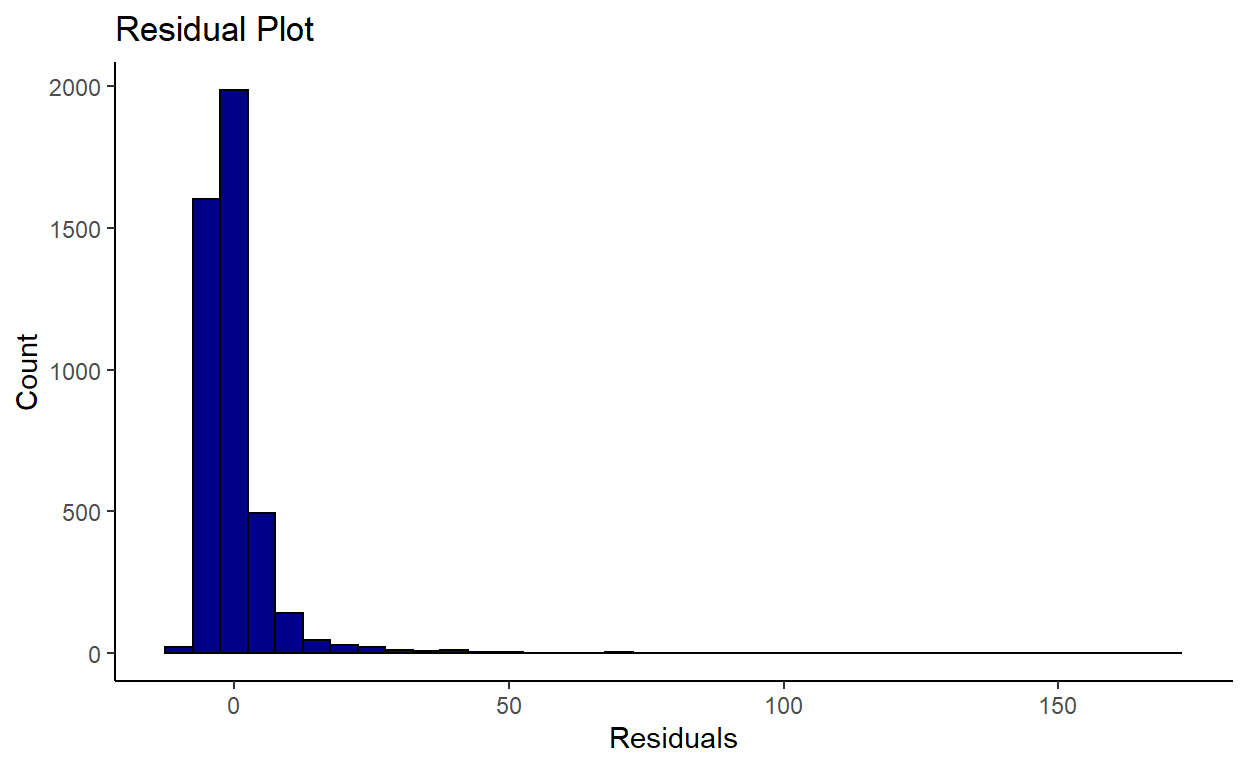
\includegraphics{sf-crime-and-hilliness_files/figure-latex/unnamed-chunk-5-1.pdf}

There is a negative correlation between \textbf{elevation} and crime. It
also appears that this relationship is not linear, so the model may fit
better if transformed. Additionally, there is a negative correlation
between \textbf{slope} and crime also showing signs of a non-linear
relationship, supporting the justification for a transformation. Lastly,
there appears to be a weak negative correlation, or even possibly no
significant relationship, between \textbf{median income} and car
break-ins.

Lastly, the figure below visualizes the spatial distribution of the
crime data within the city and provides a relative idea of the areas of
higher elevation. Crime data is distributed across most of the study
area. Additionally, regions with significant terrain (such as Twin
Peaks, Potrero Hill, and Nob Hill) can be identified by the areas with
concentrations of darker green points.

\begin{Shaded}
\begin{Highlighting}[]
\FunctionTok{tmap\_mode}\NormalTok{(}\StringTok{"view"}\NormalTok{)}

\FunctionTok{tm\_shape}\NormalTok{(crimes) }\SpecialCharTok{+}
  \FunctionTok{tm\_dots}\NormalTok{(}\StringTok{"elev"}\NormalTok{) }\SpecialCharTok{+}
  \FunctionTok{tm\_layout}\NormalTok{(}\AttributeTok{title =} \StringTok{"Figure 4. Distribution of break{-}ins by elevation"}\NormalTok{)}
\end{Highlighting}
\end{Shaded}

\hypertarget{test-ols-assumptions}{%
\subsubsection{6. Test OLS Assumptions}\label{test-ols-assumptions}}

In order to appropriately utilize an Ordinary Least Squares (OLS)
regression model, the following set of key assumptions should be met:

\begin{enumerate}
\def\labelenumi{\arabic{enumi}.}
\tightlist
\item
  The population relationship is linear in parameters with an additive
  disturbance.
\item
  Our \(X\) variables are \textbf{exogenous}, \emph{i.e.},
  \(\mathop{\boldsymbol{E}}\left[ u \mid X \right] = 0\).
\item
  The \(X\) variables have variation.
\item
  The population disturbances \(u_i\) are independently and identically
  distributed as \textbf{normal} random variables with mean zero
  \(\left( \mathop{\boldsymbol{E}}\left[ u \right] = 0 \right)\) and
  variance \(\sigma^2\) (\emph{i.e.},
  \(\mathop{\boldsymbol{E}}\left[ u^2 \right] = \sigma^2\))
\end{enumerate}

For the purpose of this analysis, Assumption \#1 holds because the
relationships observed in Figure 2 appear linear in parameters.
Additionally, this analysis claims that Assumption \#2 holds. Assumption
\#3 holds because the \(x\) variables have variation as shown in Figures
1 and 2.

Below, Assumption \#4 is tested by generating the residuals from the
main regression equation and to assess all components. The distribution
of residuals is shown in Figure 5. below:

\begin{Shaded}
\begin{Highlighting}[]
\NormalTok{crime\_lm }\OtherTok{\textless{}{-}}\NormalTok{ crimes\_summary }\SpecialCharTok{\%\textgreater{}\%} 
  \FunctionTok{add\_predictions}\NormalTok{(}\AttributeTok{model =} \FunctionTok{lm}\NormalTok{(count }\SpecialCharTok{\textasciitilde{}}\NormalTok{ elev }\SpecialCharTok{+}\NormalTok{ slope }\SpecialCharTok{+}\NormalTok{ median\_income, }\AttributeTok{data =}\NormalTok{ crimes\_summary)) }\SpecialCharTok{\%\textgreater{}\%} 
  \FunctionTok{mutate}\NormalTok{(}\AttributeTok{res =}\NormalTok{ count }\SpecialCharTok{{-}}\NormalTok{ pred)}

\FunctionTok{ggplot}\NormalTok{(}\AttributeTok{data =}\NormalTok{ crime\_lm, }\FunctionTok{aes}\NormalTok{(}\AttributeTok{x =}\NormalTok{ res)) }\SpecialCharTok{+}
  \FunctionTok{geom\_histogram}\NormalTok{(}\AttributeTok{binwidth =} \DecValTok{5}\NormalTok{, }\AttributeTok{fill =} \StringTok{"darkblue"}\NormalTok{, }\AttributeTok{col =} \StringTok{"black"}\NormalTok{) }\SpecialCharTok{+} 
  \FunctionTok{labs}\NormalTok{(}\AttributeTok{title =} \StringTok{"Figure 5. Residual Plot"}\NormalTok{,}
       \AttributeTok{x =} \StringTok{"Residuals"}\NormalTok{,}
       \AttributeTok{y =} \StringTok{"Count"}\NormalTok{) }\SpecialCharTok{+}
  \FunctionTok{theme\_classic}\NormalTok{()}
\end{Highlighting}
\end{Shaded}

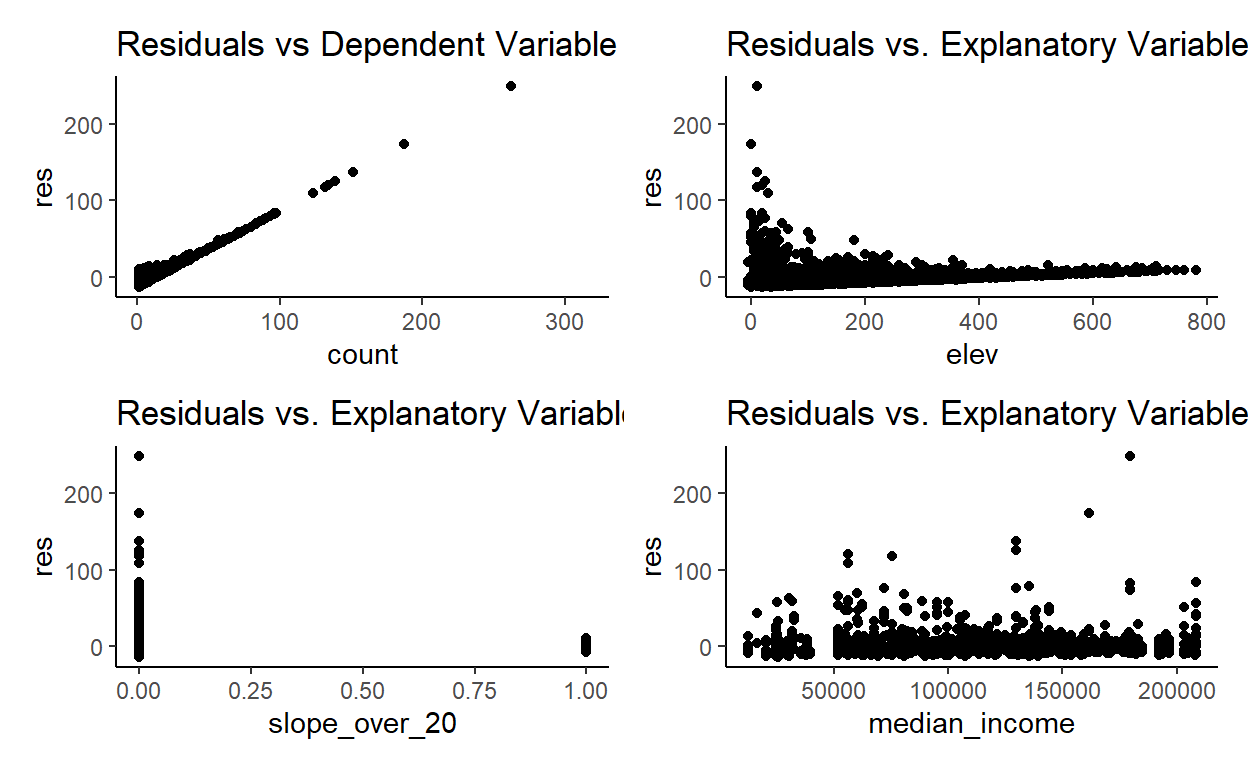
\includegraphics{sf-crime-and-hilliness_files/figure-latex/unnamed-chunk-7-1.pdf}

The residuals do not appear to be normally distributed because there is
a long right tail. This indicates that the model is over-estimating the
dependent variable for certain values of the independent variables.

Next, Figure 6 shows a QQ plot of the distribution, which visualizes the
normality of the residuals.

\begin{Shaded}
\begin{Highlighting}[]
\FunctionTok{ggplot}\NormalTok{(}\AttributeTok{data =}\NormalTok{ crime\_lm, }\FunctionTok{aes}\NormalTok{(}\AttributeTok{sample =}\NormalTok{ res)) }\SpecialCharTok{+}
  \FunctionTok{geom\_qq}\NormalTok{(}\AttributeTok{alpha =} \FloatTok{0.5}\NormalTok{, }\AttributeTok{color =} \StringTok{"magenta"}\NormalTok{) }\SpecialCharTok{+}
  \FunctionTok{geom\_qq\_line}\NormalTok{() }\SpecialCharTok{+}
  \FunctionTok{theme\_classic}\NormalTok{() }\SpecialCharTok{+}
  \FunctionTok{labs}\NormalTok{(}\AttributeTok{title =} \StringTok{"Figure 6. QQ Plot"}\NormalTok{,}
       \AttributeTok{x =} \StringTok{"Theoretical Normal Distribution"}\NormalTok{,}
       \AttributeTok{y =} \StringTok{"Analysis Residuals Distribution"}\NormalTok{)}
\end{Highlighting}
\end{Shaded}

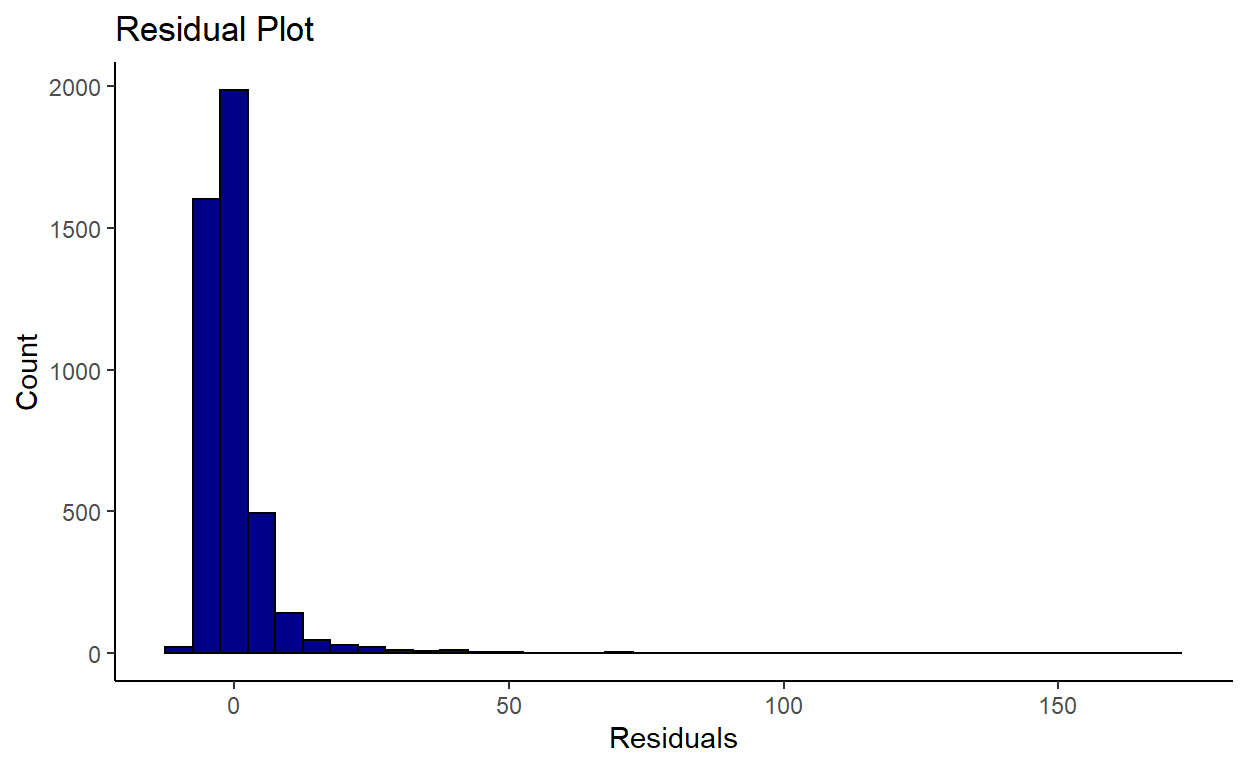
\includegraphics{sf-crime-and-hilliness_files/figure-latex/unnamed-chunk-8-1.pdf}

The QQ plot indicates that the residuals are relatively normally
distributed for values up to approximately 2 on the theoretical normal
distribution. This supports the conclusion from Figure 5 that the model
residuals are not normally distributed for high values.

Lastly, Figure 7 tests whether the residuals appear to have constant
variance when plotted against our independent variables.

\begin{Shaded}
\begin{Highlighting}[]
\NormalTok{y1 }\OtherTok{\textless{}{-}} \FunctionTok{ggplot}\NormalTok{(}\AttributeTok{data =}\NormalTok{ crime\_lm, }\FunctionTok{aes}\NormalTok{(}\AttributeTok{x =}\NormalTok{ elev, }\AttributeTok{y =}\NormalTok{ res)) }\SpecialCharTok{+}
  \FunctionTok{geom\_point}\NormalTok{(}\AttributeTok{alpha =} \FloatTok{0.25}\NormalTok{, }\AttributeTok{color =} \StringTok{"darkgreen"}\NormalTok{) }\SpecialCharTok{+} \FunctionTok{theme\_classic}\NormalTok{() }\SpecialCharTok{+} 
  \FunctionTok{labs}\NormalTok{(}\AttributeTok{title =} \StringTok{"Residuals vs. Elevation"}\NormalTok{,}
       \AttributeTok{x =} \StringTok{"Elevation (feet)"}\NormalTok{,}
       \AttributeTok{y =} \StringTok{"Residual Error"}\NormalTok{) }\SpecialCharTok{+}
  \FunctionTok{theme}\NormalTok{(}\AttributeTok{title =} \FunctionTok{element\_text}\NormalTok{(}\AttributeTok{size =} \DecValTok{10}\NormalTok{))}

\NormalTok{y2 }\OtherTok{\textless{}{-}} \FunctionTok{ggplot}\NormalTok{(}\AttributeTok{data =}\NormalTok{ crime\_lm, }\FunctionTok{aes}\NormalTok{(}\AttributeTok{x =}\NormalTok{ slope, }\AttributeTok{y =}\NormalTok{ res)) }\SpecialCharTok{+}
  \FunctionTok{geom\_point}\NormalTok{(}\AttributeTok{alpha =} \FloatTok{0.25}\NormalTok{, }\AttributeTok{color =} \StringTok{"orange"}\NormalTok{) }\SpecialCharTok{+} \FunctionTok{theme\_classic}\NormalTok{() }\SpecialCharTok{+} 
  \FunctionTok{labs}\NormalTok{(}\AttributeTok{title =} \StringTok{"Residuals vs. Slope"}\NormalTok{,}
       \AttributeTok{x =} \StringTok{"Slope (percent)"}\NormalTok{,}
       \AttributeTok{y =} \StringTok{"Residual Error"}\NormalTok{) }\SpecialCharTok{+}
  \FunctionTok{theme}\NormalTok{(}\AttributeTok{title =} \FunctionTok{element\_text}\NormalTok{(}\AttributeTok{size =} \DecValTok{10}\NormalTok{))}

\NormalTok{y3 }\OtherTok{\textless{}{-}} \FunctionTok{ggplot}\NormalTok{(}\AttributeTok{data =}\NormalTok{ crime\_lm, }\FunctionTok{aes}\NormalTok{(}\AttributeTok{x =}\NormalTok{ median\_income, }\AttributeTok{y =}\NormalTok{ res)) }\SpecialCharTok{+}
  \FunctionTok{geom\_point}\NormalTok{(}\AttributeTok{alpha =} \FloatTok{0.25}\NormalTok{, }\AttributeTok{color =} \StringTok{"blue"}\NormalTok{) }\SpecialCharTok{+} \FunctionTok{theme\_classic}\NormalTok{() }\SpecialCharTok{+} 
  \FunctionTok{labs}\NormalTok{(}\AttributeTok{title =} \StringTok{"Residuals vs. Income"}\NormalTok{,}
       \AttributeTok{x =} \StringTok{"Median Income"}\NormalTok{,}
       \AttributeTok{y =} \StringTok{"Residual Error"}\NormalTok{) }\SpecialCharTok{+}
  \FunctionTok{theme}\NormalTok{(}\AttributeTok{title =} \FunctionTok{element\_text}\NormalTok{(}\AttributeTok{size =} \DecValTok{10}\NormalTok{))}

\NormalTok{y1 }\SpecialCharTok{+}\NormalTok{ (y2 }\SpecialCharTok{/}\NormalTok{ y3) }\SpecialCharTok{+} \FunctionTok{plot\_annotation}\NormalTok{(}\AttributeTok{title =} \StringTok{\textquotesingle{}Figure 7. Residual variance across independent variables\textquotesingle{}}\NormalTok{,}
                                         \AttributeTok{theme =} \FunctionTok{theme}\NormalTok{(}\AttributeTok{plot.title =} \FunctionTok{element\_text}\NormalTok{(}\AttributeTok{hjust =} \FloatTok{0.5}\NormalTok{)))}
\end{Highlighting}
\end{Shaded}

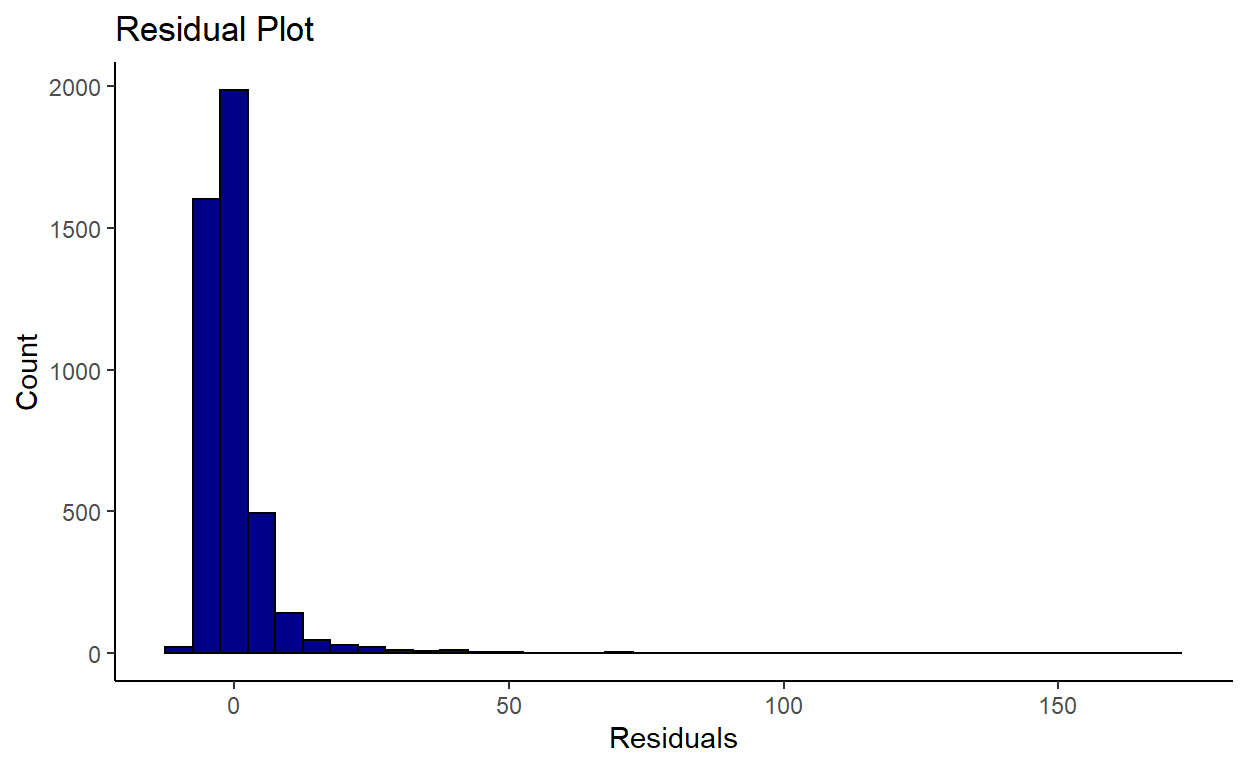
\includegraphics{sf-crime-and-hilliness_files/figure-latex/unnamed-chunk-9-1.pdf}

It does not appear that the residuals have constant variance for the
independent variables. The plots for elevation and slope have higher
variance for lower values and all three plots do not appear to be
centered at 0. Therefore, it is likely that Assumption \#4 is violated.

Since Assumptions \#1, \#2, and \#3 appear to be satisfied, in this case
using \textbf{OLS is an unbiased estimator of the coefficients}.
However, Figures 5-7 provide sufficient concern that Assumption \#4 is
not satisfied and therefore \textbf{OLS may not be the estimator with
lowest variance}. An alternative estimator to OLS may provide estimates
of the true population parameters with less variance. The analysis will
continue using OLS while taking this into account as a limitation for
the interpretation of results.

\hypertarget{regression-analysis}{%
\subsection{7. Regression Analysis}\label{regression-analysis}}

\hypertarget{model-1}{%
\subsubsection{Model 1}\label{model-1}}

Below are the results of the OLS regression analysis for the original
equation, which is repeated below:

\[NumBreakIns_i = \beta_0 + \beta_1Elevation_i + \beta_2Slope_i + \beta_3MedianIncome_i + u_i\]

\begin{Shaded}
\begin{Highlighting}[]
\NormalTok{model }\OtherTok{\textless{}{-}} \FunctionTok{lm}\NormalTok{(}\AttributeTok{formula =}\NormalTok{ count }\SpecialCharTok{\textasciitilde{}}\NormalTok{ elev }\SpecialCharTok{+}\NormalTok{ slope }\SpecialCharTok{+}\NormalTok{ median\_income, }\AttributeTok{data =}\NormalTok{ crimes\_summary)}

\FunctionTok{summ}\NormalTok{(model, }\AttributeTok{digits =} \DecValTok{7}\NormalTok{) }
\end{Highlighting}
\end{Shaded}

\begin{table}[!h]
\centering
\begin{tabular}{lr}
\toprule
\cellcolor{gray!6}{Observations} & \cellcolor{gray!6}{4391 (23 missing obs. deleted)}\\
Dependent variable & count\\
\cellcolor{gray!6}{Type} & \cellcolor{gray!6}{OLS linear regression}\\
\bottomrule
\end{tabular}
\end{table} \begin{table}[!h]
\centering
\begin{tabular}{lr}
\toprule
\cellcolor{gray!6}{F(3,4387)} & \cellcolor{gray!6}{151.4730923}\\
R² & 0.0938608\\
\cellcolor{gray!6}{Adj. R²} & \cellcolor{gray!6}{0.0932411}\\
\bottomrule
\end{tabular}
\end{table} \begin{table}[!h]
\centering
\begin{threeparttable}
\begin{tabular}{lrrrr}
\toprule
  & Est. & S.E. & t val. & p\\
\midrule
\cellcolor{gray!6}{(Intercept)} & \cellcolor{gray!6}{10.1472401} & \cellcolor{gray!6}{0.3589623} & \cellcolor{gray!6}{28.2682638} & \cellcolor{gray!6}{0.0000000}\\
elev & -0.0139627 & 0.0009376 & -14.8922804 & 0.0000000\\
\cellcolor{gray!6}{slope} & \cellcolor{gray!6}{-0.1468949} & \cellcolor{gray!6}{0.0213511} & \cellcolor{gray!6}{-6.8799698} & \cellcolor{gray!6}{0.0000000}\\
median\_income & -0.0000094 & 0.0000027 & -3.4337539 & 0.0006008\\
\bottomrule
\end{tabular}
\begin{tablenotes}
\item Standard errors: OLS
\end{tablenotes}
\end{threeparttable}
\end{table}

First, the coefficients can be interpreted from the summary above:

\begin{itemize}
\tightlist
\item
  \textbf{Intercept}: When elevation, slope, and median income are equal
  to \(0\), the expected average number of car break-ins is
  \textasciitilde10.15.
\item
  \textbf{Elevation}: With all else constant, for a 1 foot increase in
  elevation, there is a \textasciitilde0.014 decrease in the number of
  break-ins.
\item
  \textbf{Slope}: With all else constant, for a 1 percent increase in
  slope, there is a \textasciitilde0.15 decrease in the number of
  break-ins.
\item
  \textbf{Median Income}: With all else constant, for a \$1 increase in
  USD, there is a \textasciitilde0.00001 decrease in the number of
  break-ins (more intuitively, a \$10,000 increase has an expected
  decrease in break-ins of 0.1).
\end{itemize}

Next, we can interpret the significance of these coefficients using the
p-value. For all independent variables, the \textbf{p-value is less than
0.001} indicating that each of the independent variables have a
significant effect.

Lastly, the \(R^2\) value of approximately 0.09 indicates that
\textbf{\textasciitilde9\% of the variance in number of break-ins is
accounted for in the model}. This is an expectedly low result, as crime
is most likely going to be related to many other socio-economic and
demographic factors that were not considered in this analysis, such as
population density, racial composition, land use, etc. However, this
analysis singles out the possible effects of topography.

\hypertarget{model-2-logarithmic-transformation-of-dependent-variable}{%
\subsubsection{Model 2: Logarithmic transformation of dependent
variable}\label{model-2-logarithmic-transformation-of-dependent-variable}}

It is also important to compare the results of the OLS analysis with an
alternative regression equation. In earlier sections, it was identified
that the relationship of both elevation and slope with break-ins
appeared to be non-linear. Therefore, it could be appropriate to
transform the equation. The equation and summary below demonstrate the
different results when log-transforming the dependent variable.

\[log(NumBreakIns_i) = \beta_0 + \beta_1Elevation_i + \beta_2Slope_i + \beta_3MedianIncome_i + u_i\]

\begin{Shaded}
\begin{Highlighting}[]
\NormalTok{model\_transformed }\OtherTok{\textless{}{-}} \FunctionTok{lm}\NormalTok{(}\AttributeTok{formula =} \FunctionTok{log}\NormalTok{(count) }\SpecialCharTok{\textasciitilde{}}\NormalTok{ elev }\SpecialCharTok{+}\NormalTok{ slope }\SpecialCharTok{+}\NormalTok{ median\_income, }\AttributeTok{data =}\NormalTok{ crimes\_summary)}

\FunctionTok{summ}\NormalTok{(model\_transformed, }\AttributeTok{digits =} \DecValTok{7}\NormalTok{)}
\end{Highlighting}
\end{Shaded}

\begin{table}[!h]
\centering
\begin{tabular}{lr}
\toprule
\cellcolor{gray!6}{Observations} & \cellcolor{gray!6}{4391 (23 missing obs. deleted)}\\
Dependent variable & log(count)\\
\cellcolor{gray!6}{Type} & \cellcolor{gray!6}{OLS linear regression}\\
\bottomrule
\end{tabular}
\end{table} \begin{table}[!h]
\centering
\begin{tabular}{lr}
\toprule
\cellcolor{gray!6}{F(3,4387)} & \cellcolor{gray!6}{247.6027651}\\
R² & 0.1448023\\
\cellcolor{gray!6}{Adj. R²} & \cellcolor{gray!6}{0.1442175}\\
\bottomrule
\end{tabular}
\end{table} \begin{table}[!h]
\centering
\begin{threeparttable}
\begin{tabular}{lrrrr}
\toprule
  & Est. & S.E. & t val. & p\\
\midrule
\cellcolor{gray!6}{(Intercept)} & \cellcolor{gray!6}{1.8826251} & \cellcolor{gray!6}{0.0391027} & \cellcolor{gray!6}{48.1456352} & \cellcolor{gray!6}{0.0000000}\\
elev & -0.0019118 & 0.0001021 & -18.7187543 & 0.0000000\\
\cellcolor{gray!6}{slope} & \cellcolor{gray!6}{-0.0211530} & \cellcolor{gray!6}{0.0023258} & \cellcolor{gray!6}{-9.0948218} & \cellcolor{gray!6}{0.0000000}\\
median\_income & -0.0000014 & 0.0000003 & -4.6866190 & 0.0000029\\
\bottomrule
\end{tabular}
\begin{tablenotes}
\item Standard errors: OLS
\end{tablenotes}
\end{threeparttable}
\end{table}

The \(R^2\) value for Model 2 of 0.145 is higher than the previous
\(R^2\) of 0.09 for Model 1. This indicates that \textbf{a
transformation may be a better model fit} for the data.

\hypertarget{model-3-transformation-of-independent-variables}{%
\subsubsection{Model 3: Transformation of independent
variables}\label{model-3-transformation-of-independent-variables}}

Another method of transforming the regression equation to deal with
non-linear relationships is to log-transform the two independent
variables, slope and elevation, which appeared to have non-linear
relationships with break-ins.

\[NumBreakIns_i = \beta_0 + \beta_1*log(Elevation_i) + \beta_2*log(Slope_i) + \beta_3MedianIncome_i + u_i\]

\begin{Shaded}
\begin{Highlighting}[]
\NormalTok{crimes\_transformed }\OtherTok{\textless{}{-}}\NormalTok{ crimes\_summary }\SpecialCharTok{\%\textgreater{}\%}
  \FunctionTok{mutate}\NormalTok{(}\AttributeTok{elev =} \FunctionTok{case\_when}\NormalTok{(elev }\SpecialCharTok{==} \SpecialCharTok{{-}}\DecValTok{5} \SpecialCharTok{\textasciitilde{}} \DecValTok{0}\NormalTok{,}
                          \ConstantTok{TRUE} \SpecialCharTok{\textasciitilde{}}\NormalTok{ elev)) }\SpecialCharTok{\%\textgreater{}\%} 
  \FunctionTok{mutate}\NormalTok{(}\AttributeTok{elev\_shift =}\NormalTok{ elev }\SpecialCharTok{+} \FloatTok{0.01}\NormalTok{,}
         \AttributeTok{slope\_shift =}\NormalTok{ slope }\SpecialCharTok{+} \FloatTok{0.01}\NormalTok{)}

\NormalTok{model\_indeptransformed }\OtherTok{\textless{}{-}} \FunctionTok{lm}\NormalTok{(}\AttributeTok{formula =}\NormalTok{ count }\SpecialCharTok{\textasciitilde{}} \FunctionTok{log}\NormalTok{(elev\_shift) }\SpecialCharTok{+} \FunctionTok{log}\NormalTok{(slope\_shift) }\SpecialCharTok{+}\NormalTok{ median\_income, }\AttributeTok{data =}\NormalTok{ crimes\_transformed)}

\FunctionTok{summ}\NormalTok{(model\_indeptransformed, }\AttributeTok{digits =} \DecValTok{7}\NormalTok{)}
\end{Highlighting}
\end{Shaded}

\begin{table}[!h]
\centering
\begin{tabular}{lr}
\toprule
\cellcolor{gray!6}{Observations} & \cellcolor{gray!6}{4391 (23 missing obs. deleted)}\\
Dependent variable & count\\
\cellcolor{gray!6}{Type} & \cellcolor{gray!6}{OLS linear regression}\\
\bottomrule
\end{tabular}
\end{table} \begin{table}[!h]
\centering
\begin{tabular}{lr}
\toprule
\cellcolor{gray!6}{F(3,4387)} & \cellcolor{gray!6}{253.8109749}\\
R² & 0.1478961\\
\cellcolor{gray!6}{Adj. R²} & \cellcolor{gray!6}{0.1473134}\\
\bottomrule
\end{tabular}
\end{table} \begin{table}[!h]
\centering
\begin{threeparttable}
\begin{tabular}{lrrrr}
\toprule
  & Est. & S.E. & t val. & p\\
\midrule
\cellcolor{gray!6}{(Intercept)} & \cellcolor{gray!6}{17.3094410} & \cellcolor{gray!6}{0.4958695} & \cellcolor{gray!6}{34.9072477} & \cellcolor{gray!6}{0.0000000}\\
log(elev\_shift) & -1.9343470 & 0.0913324 & -21.1791979 & 0.0000000\\
\cellcolor{gray!6}{log(slope\_shift)} & \cellcolor{gray!6}{-0.6571915} & \cellcolor{gray!6}{0.0957164} & \cellcolor{gray!6}{-6.8660252} & \cellcolor{gray!6}{0.0000000}\\
median\_income & -0.0000133 & 0.0000026 & -5.1502651 & 0.0000003\\
\bottomrule
\end{tabular}
\begin{tablenotes}
\item Standard errors: OLS
\end{tablenotes}
\end{threeparttable}
\end{table}

The \(R^2\) value for Model 3 of 0.148 is slightly higher still than
Model 2, with all coefficients still similarly statistically
significant.

\hypertarget{interpret-results}{%
\subsection{8. Interpret Results}\label{interpret-results}}

In conclusion, the linear regression model predicts that \textbf{there
are significant negative relationships between the key independent
variables (slope and elevation) and the dependent variable (number of
car break-ins)}. While there is a statistically significant relationship
with median income, the effect size is seemingly negligible. It was also
found that transformations result in better model fit because the
non-linear relationships are more accurately taken into account.

The study found that certain assumptions of OLS were violated, meaning
that \textbf{the OLS method is most likely not the estimator with lowest
variance.} This needs to be taken into account while interpreting the
resulting coefficients of the variables.

This analysis has room for improvement, including but not limited to: 1.
Ensuring that the OLS assumption violation is solved by the
transformation of the data or by using another estimator. 2. Including
key socio-economic and demographic variables with more significant
correlation than median income. 3. More thoroughly researching and
selecting the proper transformation method.

All code for this analysis can be found on
\href{https://github.com/alexclippinger/alexclippinger.github.io/blob/main/_posts/2021-11-02-sf-crime-and-hilliness/sf-crime-and-hilliness.Rmd}{\textbf{GitHub}}.

\hypertarget{refs}{}
\begin{CSLReferences}{1}{0}
\leavevmode\hypertarget{ref-sfdata}{}%
City, and County of San Francisco. 2021.
{``DataSF.''}\url{\%20\%0A\%20\%20\%20\%20\%20\%20\%20\%20https://datasf.org/\%0A\%20\%20\%20\%20\%0A}.

\leavevmode\hypertarget{ref-sfcrime}{}%
Kim, Young-An, and James C. Wo. 2021. {``Topography and Crime in Place:
The Effects of Elevation, Slope, and Betweenness in San Francisco Street
Segments.''} \emph{Journal of Urban Affairs}, 1--25.
\url{https://doi.org/10.1080/07352166.2021.1901591}.

\leavevmode\hypertarget{ref-tidycensus}{}%
Walker, Kyle. 2021. {``Tidycensus: Load US Census Boundary and Attribute
Data as 'Tidyverse' and 'Sf'-Ready Data
Frames.''}\url{\%20\%0A\%20\%20\%20\%20\%20\%20\%20\%20https://CRAN.R-project.org/package=tidycensus\%0A\%20\%20\%20\%20\%0A}.

\end{CSLReferences}

\end{document}
